\documentclass[a4paper]{article}

\usepackage{lcutrinko}

\usepackage[top=10truemm,bottom=15truemm,left=10truemm,right=10truemm,headheight=0truemm,headsep=0truemm,footskip=10truemm]{geometry}

\usepackage{tabularx}
\usepackage{graphicx}

\begin{document}

\title{A Study of Denkikei's History}
\date{January 1st, 1873}
\author{01-234567 Taro Denki}
\rinkotype{Survey Report}
\laboratory{Supervisor: Prof. William Edward Ayrton}

\dendentitle

\begin{abstract}
  ``Todai Denkikei''(\textit{T\^odai Denkik\^e}) derives from Department of Telegraphy in Imperial College of Engineering, Ministry of Industry (\textit{K\^obush\^o K\^ogakury\^o Denshinka}) established in 1873.
\end{abstract}

\section{Recent Events}

Table~\ref{tab:events} shows some important events of Denkikei in this century.

\begin{table}[htbp]
  \centering
  \caption{Some important events of Denkikei in this century}
  \label{tab:events}
  \begin{tabularx}{\linewidth}{r|X}
    Year & Event \\ \hline
    2001 & Department of Information and Communication Engineering established in Graduate School of Information Science and Technology\\
    2005 & Engineering Bldg. \#2 completed\\
    2008 & Department of Electrical Engineering and Information Systems established (created by reforming Department of Electrical Engineering, Department of Electronics Engineering, and Department of Frontier Informatics)\\
    2009 & Undergraduate Department of Electrical and Electronics Engineering established \\
  \end{tabularx}
\end{table}

\section{Professor Ayrton}

Dr. William Edward Ayrton (Fig.~\ref{fig:ayrton}) is the first professor of Denkikei.

\begin{figure}[htbp]
  \centering
  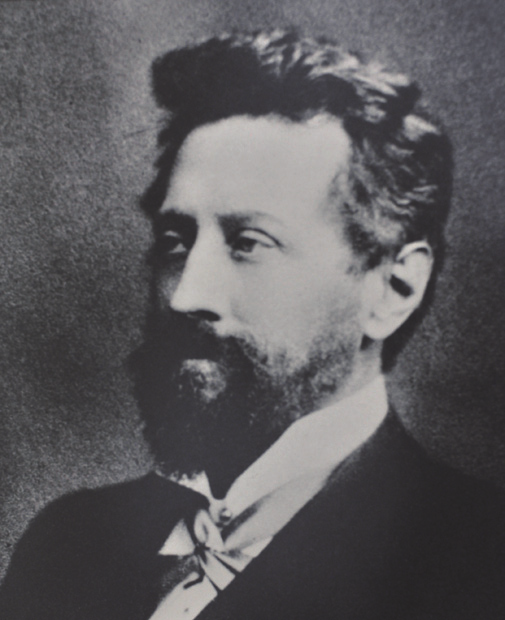
\includegraphics[height=45truemm]{ayrton.png}
  \caption{Prof. W. E. Ayrton}
  \label{fig:ayrton}
\end{figure}

\begin{thebibliography}{9}
\bibitem{guidance} Office of Denkikei, Faculty of Engineering, the University of Tokyo ``Shingaku Guidance Book 2016'' (Japanese)
\end{thebibliography}


\end{document}